\documentclass[a4paper]{article}
\usepackage{listings}
\usepackage{geometry}
\usepackage[parfill]{parskip}
\usepackage[bottom]{footmisc}

\usepackage[bookmarks=true, bookmarksopen=true]{hyperref}
\usepackage{bookmark}
\usepackage{enumitem}
\usepackage{color}
\definecolor{linkcolour}{rgb}{0,0.2,0.6}
\hypersetup{colorlinks, breaklinks, urlcolor=linkcolour, linkcolor=linkcolour}

\usepackage{amsmath, bm}
\newcommand{\norm}[1]{\left\lVert#1\right\rVert}

\usepackage{csvsimple}

% Font
\usepackage{fontspec}
\setmainfont{GFS Artemisia}

\renewcommand{\figureautorefname}{Σχήμα}
\renewcommand{\tableautorefname}{Πίνακας}

% Images
\usepackage{graphicx}
\graphicspath{{../../figures/spectral/}}
\usepackage[font={footnotesize,it}]{caption}
\usepackage[font={footnotesize}]{subcaption}
\renewcommand{\thesubfigure}{\Roman{subfigure}}
\usepackage{float}

% for diagonal table cell
\usepackage{diagbox}

% English-Greek use
\usepackage{polyglossia}
\setmainlanguage{greek}
\setotherlanguage{english}

\geometry{
 a4paper,
 total={170mm,257mm},
 left=20mm,
 top=20mm,
}

\title{Υπολογιστική Νοημοσύνη - Στατιστική μάθηση \\ Τρίτη Εργασία}
\author{Κωστινούδης Ευάγγελος \\ΑΕΜ: 112}
\date{\today}

\begin{document}
\maketitle
\pagenumbering{gobble}
\newpage
\pagenumbering{arabic}

\section{Περιγραφή προβλήματος που επιλέχτηκε}

Για την εργασία αυτή επιλέχτηκε το πρόβλημα του διαχωρισμού κλάσεων και τα
δεδομένα προέρχονται από τις βάσεις:

\begin{enumerate}
\item \href{http://yann.lecun.com/exdb/mnist/}{MNIST}
\item \href{https://www.cs.toronto.edu/~kriz/cifar.html}{Cifar-10}
\end{enumerate}


\section{Υλοποίηση}

Η υλοποίηση του αλγορίθμου του spectral clustering που παράγει τα embeddings
βρίσκεται στο αρχείο \textit{spectral\_embeddings.py}.

Για την εκπαίδευση των μοντέλων χρησιμοποιούνται τα δεδομένα εκπαίδευσης που
δίνονται από τις δύο βάσεις που αναφέρονται παραπάνω. Επίσης, επιλέχτηκε ο
αλγόριθμος \textbf{t-SNE} για την μείωση στις δύο διαστάσεις.

\subsection{Προεπεξεργασία δεδομένων}

Η μόνη προεπεξεργασία που έγινε στα δεδομένα πριν την χρήση τους είναι ο
μετασχηματισμός των δεδομένων στο διάστημα $[0,1]$ για κάθε χαρακτηριστικό των
δεδομένων.

\subsection{Επιλογή παραμέτρων}
\subsubsection{Παράμετροι του t-SNE}

Και για τις δύο βάσεις ελέγχθηκαν οι τιμές του perplexity $[10, 20, 30, 40, 50,
60]$.

\subsubsection{Παράμετροι του spectral clustering}

Για τον αλγόριθμο του spectral clustering για τη δημιουργία του similarity
matrix χρησιμοποιήθηκε ο αλγόριθμος των πλησιέστερων γειτόνων επειδή μπορεί να
αναπαρασταθεί με αραιό πίνακα σε σχέση με τις μεθόδους των πυρήνων. Με αυτό τον
τρόπο είναι δυνατό να τρέξει ο αλγόριθμος σε όλα τα δεδομένα, χωρίς να
χρειάζεται πάρα πολύ μνήμη.

Επίσης, για τον αλγόριθμο αυτό χρησιμοποιθήκε η κανονική μορφή του λαπλασιανού
πίνακα και όχι η κανονικοποιημένη. Ακόμα, επειδή το ιδιοδιάνυσμα που αντιστοιχεί
στην ιδιοτιμή 0 έχει όλες τις τιμές του ίδιες, δεν χρησιμοποιήθηκε.

Για τον αλγόριθμο του spectral clustering οι υπερπαράμετροι που υπάρχουν είναι ο
αριθμός των γειτόνων και ο αριθμός των embeddings που επιστρέφει τελικά ο
αλγόριθμος.

Συγκεκριμένα για τη βάση MNIST ελέγχθηκαν οι τιμές για του γείτονες $[15, 20,
25, 30, 35, 40, 50]$ και οι τιμές των embeddings $[3, 5, 8, 10, 15, 20, 30,
40]$.

Για τη βάση Cifar-10 ελέγχθηκαν οι τιμές για του γείτονες $[10, 15, 20, 25, 30,
40, 50]$ και οι τιμές των embeddings $[3, 5, 8, 10, 15, 20, 30, 40]$.

Για την επιλογή των καλύτερων παραμέτρων, έγινε ομαδοποίηση με δέκα ομάδες και
τα αποτελέσματα συγκρίθηκαν βάση της μετρικής Adjusted Rand Index (ARI) όπου
συγκρίνονται τα αποτελέσματα της ομαδοποίησης με τις πραγματικές κλάσεις των
δεδομένων. Η μετρική αυτή δίνει τιμές κοντά στο μηδέν, όταν τα αποτελέσματα
είναι τυχαία, κοντά στο 1 όταν οι ομαδοποιήσεις ταιριάζουν. Επίσης, μπορεί να
πάρει και αρνητικές τιμές όταν τα αποτελέσματα είναι χειρότερα από τα τυχαία.

\section{Αποτελέσματα}

Τα πειράματα εκτελέστηκαν σε επεξεργαστή Intel i7-4510U και 8GB μνήμη.


\subsection{Επιλογή παραμέτρων t-SNE}

\subsubsection{MNIST}

Στο \autoref{fig:mnist_tsne_all} παρουσιάζονται τα αποτελέσματα του αλγορίθμου
t-SNE για διάφορες τιμές του perplexity. Παρατηρείται ότι είναι παραπλήσια.
Επιλέχθηκε η τιμή 10 για το perplexity.

\begin{figure}[H]
    \centering
    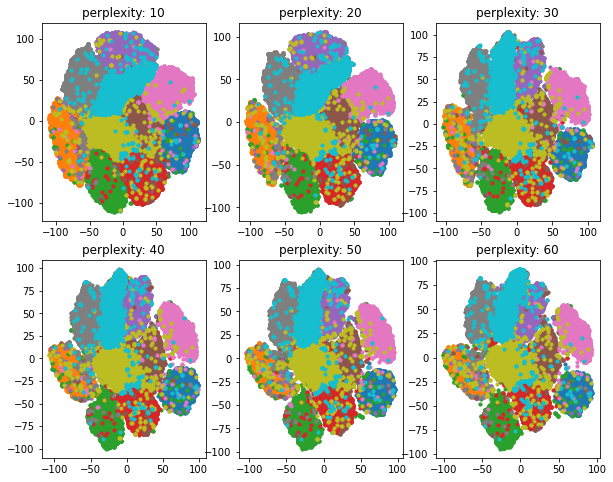
\includegraphics[width=0.6\linewidth]{mnist/tsne_all.png}
    \caption{Αποτελέσματα του t-SNE για διάφορες τιμές του perplexity για τη
    βάση MNIST.}
    \label{fig:mnist_tsne_all}
\end{figure}

Ο χρόνος εκτέλεσης για τις τιμές του perplexity που χρησιμοποιήθηκαν βρίσκονται
στον \autoref{tab:mnist_tsne_times}.

\begin{table}[H]
\centering
\begin{tabular}{|c|c|c|c|c|c|c|}
\hline
\textbf{perplexity} & \textbf{10} & \textbf{20} & \textbf{30} & \textbf{40} & \textbf{50} & \textbf{60} \\ \hline
\textbf{seconds}    & 807,75      & 962,41      & 978,5       & 910,81      & 957,05      & 1058,15     \\ \hline
\end{tabular}
\caption{Χρόνος εκτέλεσης του αλγορίθμου t-SNE για διάφορες τιμές του perplexity
    για τη βάση MNIST.}
\label{tab:mnist_tsne_times}
\end{table}

Το τελικό αποτέλεσμα στις δύο διαστάσεις παρουσιάζεται στο
\autoref{fig:mnist_tsne}.

\begin{figure}[H]
    \centering
    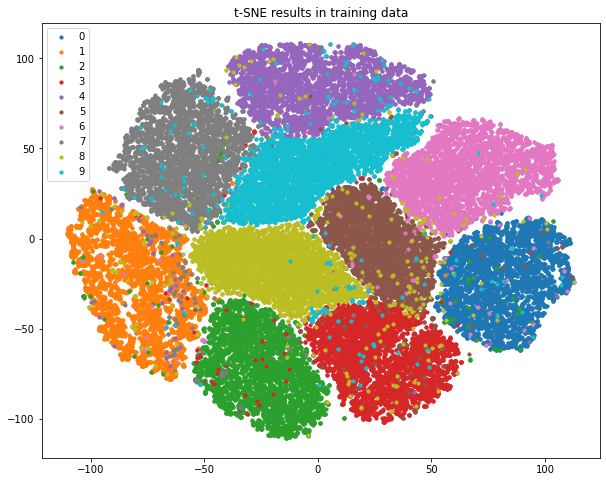
\includegraphics[width=0.6\linewidth]{mnist/tsne_training.png}
    \caption{Αποτελέσμα του t-SNE για την τιμή 10 του perplexity για τη βάση
    MNIST.}
    \label{fig:mnist_tsne}
\end{figure}

\subsubsection{Cifar-10}

Στο \autoref{fig:cifar_tsne_all} παρουσιάζονται τα αποτελέσματα του αλγορίθμου
t-SNE για διάφορες τιμές του perplexity. Παρατηρείται ότι ο αλγόριθμος αδυνατεί
να ξεχωρίσει τις κλάσεις. Επιλέχθηκε η τιμή 60 για το perplexity.

\begin{figure}[H]
    \centering
    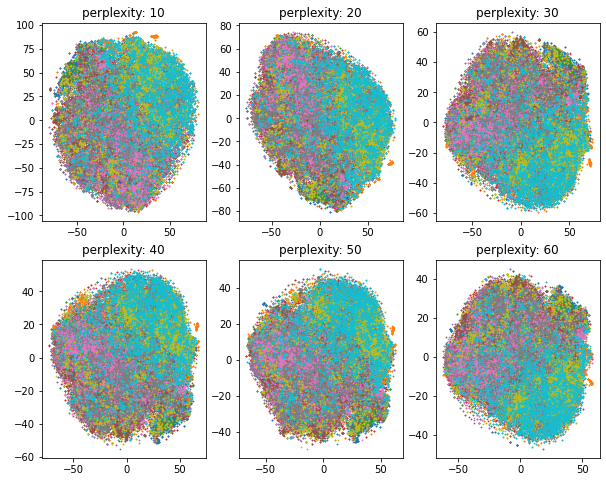
\includegraphics[width=0.6\linewidth]{cifar/tsne_all.png}
    \caption{Αποτελέσματα του t-SNE για διάφορες τιμές του perplexity για τη
    βάση Cifar-10.}
    \label{fig:cifar_tsne_all}
\end{figure}

Ο χρόνος εκτέλεσης για τις τιμές του perplexity που χρησιμοποιήθηκαν βρίσκονται
στον \autoref{tab:cifar_tsne_times}.

\begin{table}[H]
\centering
\begin{tabular}{|c|c|c|c|c|c|c|}
\hline
\textbf{perplexity} & \textbf{10} & \textbf{20} & \textbf{30} & \textbf{40} & \textbf{50} & \textbf{60} \\ \hline
\textbf{seconds}    & 1024,3      & 1059,65     & 1240,23     & 1337,87     & 1399,87     & 1418,55     \\ \hline
\end{tabular}
\caption{Χρόνος εκτέλεσης του αλγορίθμου t-SNE για διάφορες τιμές του perplexity
    για τη βάση Cifar-10.}
\label{tab:cifar_tsne_times}
\end{table}

Το τελικό αποτέλεσμα στις δύο διαστάσεις παρουσιάζεται στο
\autoref{fig:cifar_tsne}.

\begin{figure}[H]
    \centering
    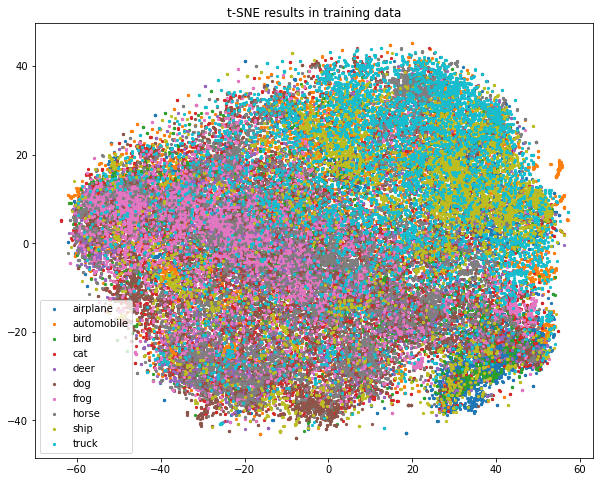
\includegraphics[width=0.6\linewidth]{cifar/tsne_training.png}
    \caption{Αποτελέσμα του t-SNE για την τιμή 10 του perplexity για τη βάση
    Cifar-10.}
    \label{fig:cifar_tsne}
\end{figure}

\subsubsection{Επιλογή παραμέτρων του spectral clustering}

\subsubsection{MNIST}

Τα αποτελέσματα της αναζήτησης πλέγματος για την επιλογή των παραμέτρων του
spectral clustering δίνονται στον \autoref{tab:mnist_grid}. Παρατηρούμε ότι το
καλύτερο αποτέλεσμα δίνεται για 50 γείτονες και 3 embeddings.

\begin{table}[H]
\centering
\begin{tabular}{|c|c|c|c|c|c|c|c|c|}
\hline
\diagbox[innerwidth=3cm]{\textbf{neightbors}}{\textbf{embeddings}} & \textbf{3} & \textbf{5} & \textbf{8} & \textbf{10} & \textbf{15} & \textbf{20} & \textbf{30} & \textbf{40} \\ \hline
\textbf{15}                                                        & 0,4422     & 0,4995     & 0,6873     & 0,48        & 0,5264      & 0,5454      & 0,3636      & 0,2594      \\ \hline
\textbf{20}                                                        & 0,7461     & 0,6794     & 0,6415     & 0,5709      & 0,6111      & 0,445       & 0,4842      & 0,3278      \\ \hline
\textbf{25}                                                        & 0,7483     & 0,6521     & 0,6004     & 0,5625      & 0,4925      & 0,551       & 0,301       & 0,2694      \\ \hline
\textbf{30}                                                        & 0,7074     & 0,7641     & 0,5954     & 0,5723      & 0,574       & 0,575       & 0,3413      & 0,3748      \\ \hline
\textbf{35}                                                        & 0,7118     & 0,6824     & 0,5969     & 0,621       & 0,5512      & 0,4322      & 0,3866      & 0,3417      \\ \hline
\textbf{40}                                                        & 0,6518     & 0,7695     & 0,6758     & 0,5682      & 0,4976      & 0,5028      & 0,3827      & 0,2743      \\ \hline
\textbf{50}                                                        & 0,8213     & 0,7845     & 0,674      & 0,6495      & 0,4559      & 0,5478      & 0,3847      & 0,4644      \\ \hline
\end{tabular}
\caption{Αποτελέσματα αναζήτησης πλέγματος της μετρικής ARI για διάφορες τιμές
    των γειτόνων και του αριθμού των embeddings για τη βάση MNIST.}
\label{tab:mnist_grid}
\end{table}


\subsubsection{Cifar-10}

Τα αποτελέσματα της αναζήτησης πλέγματος για την επιλογή των παραμέτρων του
spectral clustering δίνονται στον \autoref{tab:cifar_grid}. Παρατηρούμε ότι το
καλύτερο αποτέλεσμα δίνεται για 15 γείτονες και 20 embeddings.

\begin{table}[H]
\centering
\begin{tabular}{|c|c|c|c|c|c|c|c|c|}
\hline
\diagbox[innerwidth=3cm]{\textbf{neightbors}}{\textbf{embeddings}} & \textbf{3} & \textbf{5} & \textbf{8} & \textbf{10} & \textbf{15} & \textbf{20} & \textbf{30} & \textbf{40} \\ \hline
\textbf{10}                                                        & 0,0303     & 0,0475     & 0,0461     & 0,0414      & 0,0379      & 0,0392      & 0,0378      & 0,0311      \\ \hline
\textbf{15}                                                        & 0,0486     & 0,0457     & 0,0476     & 0,0417      & 0,04        & 0,0488      & 0,0303      & 0,0281      \\ \hline
\textbf{20}                                                        & 0,0464     & 0,0456     & 0,0483     & 0,0413      & 0,0374      & 0,0449      & 0,0356      & 0,0272      \\ \hline
\textbf{25}                                                        & 0,0473     & 0,0456     & 0,0472     & 0,0413      & 0,0367      & 0,0351      & 0,0367      & 0,0124      \\ \hline
\textbf{30}                                                        & 0,0468     & 0,046      & 0,0416     & 0,0413      & 0,0364      & 0,0362      & 0,035       & 0,0275      \\ \hline
\textbf{40}                                                        & 0,0485     & 0,0447     & 0,0474     & 0,0481      & 0,0427      & 0,0482      & 0,0351      & 0,0253      \\ \hline
\textbf{50}                                                        & 0,0449     & 0,0459     & 0,0402     & 0,0403      & 0,0362      & 0,0354      & 0,029       & 0,023       \\ \hline
\end{tabular}
\caption{Αποτελέσματα αναζήτησης πλέγματος της μετρικής ARI για διάφορες τιμές
    των γειτόνων και του αριθμού των embeddings για τη βάση Cifar-10.}
\label{tab:cifar_grid}
\end{table}


\subsubsection{Αποτελέσματα καλύτερων μοντέλων}

\subsubsection{MNIST}

Στο \autoref{fig:mnist_best_model_results} παρουσιάζεται το αποτέλεσμα της
ομαδοποίησης για 10 ομάδες τους καλύτερου μοντέλου σε σχέση με τις πραγματικές
κλάσεις. Παρατηρούμε ότι ο αλγόριθμος βρίσκει τις σωστές ομάδες, ωστόσο υπάρχουν
λάθη στα όρια μεταξύ ομάδων.

\begin{figure}[H]
    \centering
    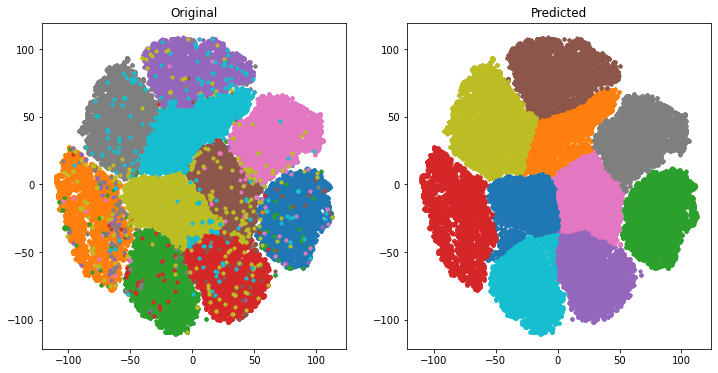
\includegraphics[width=0.6\linewidth]{mnist/best_model_results.png}
    \caption{Αποτέλεσμα ομαδοποίησης του καλύτερου μοντέλου σε σχέση με τις
    πραγματικές κλάσεις για τη βάση MNIST.}
    \label{fig:mnist_best_model_results}
\end{figure}

Στο \autoref{fig:mnist_eigenvalues} παρουσιάζονται οι 41 μικρότερες ιδιοτιμές
του καλύτερου μοντέλου. Παρατηρούμε ότι με μεγαλύτερα κενά παρουσιάζονται για
τις τιμές 8, 21, 26.

\begin{figure}[H]
    \centering
    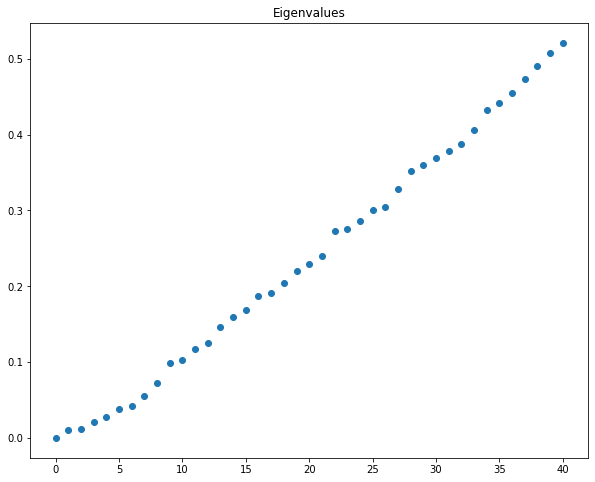
\includegraphics[width=0.6\linewidth]{mnist/eigenvalues.png}
    \caption{Ιδιοτιμές του καλύτερου μοντέλου για τη βάση MNIST.}
    \label{fig:mnist_eigenvalues}
\end{figure}

Τέλος, παρουσιάζονται τα αποτελέσματα για τους αριθμούς των ομάδων $[10, 15, 20,
25, 30, 40]$. Στο \autoref{fig:mnist_dif_clusters} παρουσιάζονται τα
αποτελέσματα για τις ομάδες αυτές. Στον \autoref{tab:mnist_sil} παρουσιάζεται η
μετρική silhouette με βάση τις αποστάσεις των embeddings και τις αποστάσεις στις
δύο διαστάσεις (που παρήγαγε ο t-SNE).

Από το \autoref{fig:mnist_dif_clusters} παρατηρούμε ότι όσο μεγαλύνει ο αριθμός
των ομάδων τόσο οι ομάδες χωρίζονται, εκτός από τις δύο ομάδες πάνω δεξιά που
μένουν σχεδόν αναλλοίωτες.

Από τον \autoref{tab:mnist_sil} παρατηρούμε ότι το καλύτερο αποτέλεσμα βάση της
μετρικής silhouette είναι για 10 ομάδες.

\begin{figure}[H]
    \centering
    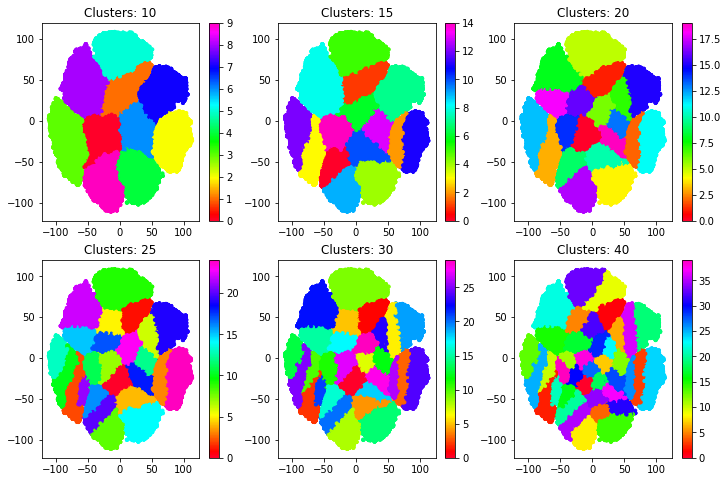
\includegraphics[width=0.6\linewidth]{mnist/dif_clusters.png}
    \caption{Αποτελέσματα για διάφορες τιμές του αριθμού των ομάδων για τη βάση
    MNIST.}
    \label{fig:mnist_dif_clusters}
\end{figure}

\begin{table}[H]
\centering
\begin{tabular}{|c|c|c|c|c|c|c|}
\hline
\diagbox[innerwidth=3cm]{\textbf{Data}}{\textbf{Clusters}} & \textbf{10} & \textbf{15} & \textbf{20} & \textbf{25} & \textbf{30} & \textbf{40} \\ \hline
\textbf{Embeddings}                                        & 0,5244      & 0,5023      & 0,4926      & 0,4699      & 0,4492      & 0,4159      \\ \hline
\textbf{TSNE 2D space}                                     & 0,3632      & 0,3067      & 0,2639      & 0,258       & 0,257       & 0,2564      \\ \hline
\end{tabular}
\caption{Αποτελέσματα μετρικής silhouette με βάση τις αποστάσεις των embeddings
    και τις αποστάσεις στις δύο διαστάσεις για τη βάση MNIST.}
\label{tab:mnist_sil}
\end{table}

\subsubsection{Cifar-10}

Στο \autoref{fig:cifar_best_model_results} παρουσιάζεται το αποτέλεσμα της
ομαδοποίησης για 10 ομάδες τους καλύτερου μοντέλου σε σχέση με τις πραγματικές
κλάσεις. Παρατηρούμε ότι ο αλγόριθμος δεν βρίσκει τις ομάδες όπως είναι, γεγονός
που είναι αναμενόμενο αφού δεν υπάρχει κάποιο διαχωρισμός των ομάδων.

\begin{figure}[H]
    \centering
    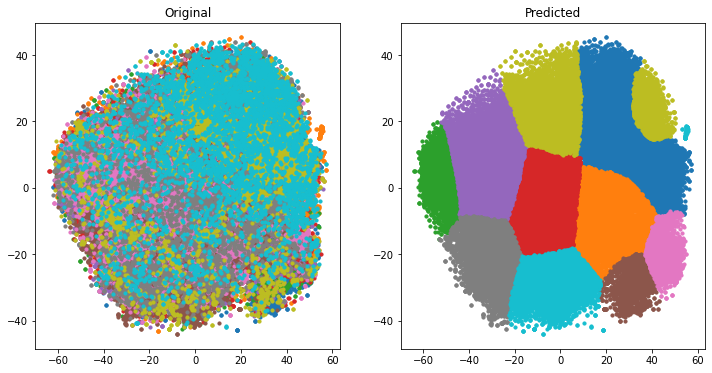
\includegraphics[width=0.6\linewidth]{cifar/best_model_results.png}
    \caption{Αποτέλεσμα ομαδοποίησης του καλύτερου μοντέλου σε σχέση με τις
    πραγματικές κλάσεις για τη βάση Cifar-10.}
    \label{fig:cifar_best_model_results}
\end{figure}

Στο \autoref{fig:cifar_eigenvalues} παρουσιάζονται οι 41 μικρότερες ιδιοτιμές
του καλύτερου μοντέλου. Παρατηρούμε ότι με μεγαλύτερα κενά παρουσιάζονται για
τις τιμές 5, 16, 21, 37.

\begin{figure}[H]
    \centering
    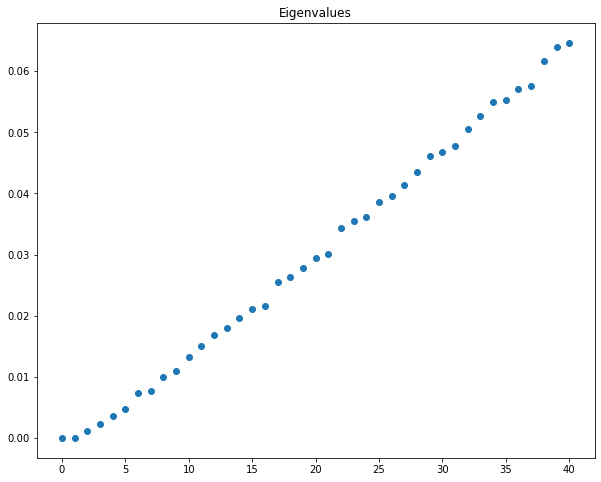
\includegraphics[width=0.6\linewidth]{cifar/eigenvalues.png}
    \caption{Ιδιοτιμές του καλύτερου μοντέλου για τη βάση Cifar-10.}
    \label{fig:cifar_eigenvalues}
\end{figure}

Τέλος, παρουσιάζονται τα αποτελέσματα για τους αριθμούς των ομάδων $[10, 15, 20,
25, 30, 40]$. Στο \autoref{fig:cifar_dif_clusters} παρουσιάζονται τα
αποτελέσματα για τις ομάδες αυτές. Στον \autoref{tab:cifar_sil} παρουσιάζεται η
μετρική silhouette με βάση τις αποστάσεις των embeddings και τις αποστάσεις στις
δύο διαστάσεις (που παρήγαγε ο t-SNE).

Από το \autoref{fig:cifar_dif_clusters} παρατηρούμε ότι όσο μεγαλύνει ο αριθμός
των ομάδων τόσο οι ομάδες χωρίζονται ομοιόμορφα.

Από τον \autoref{tab:cifar_sil} παρατηρούμε ότι το καλύτερο αποτέλεσμα βάση της
μετρικής silhouette είναι για 10 ομάδες.

\begin{figure}[H]
    \centering
    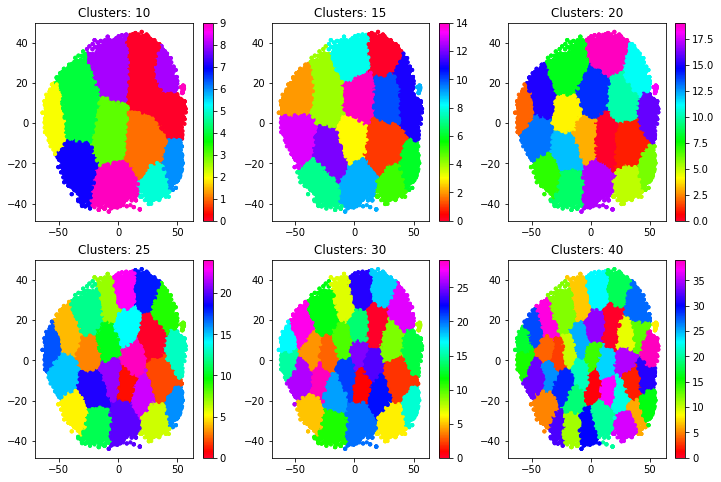
\includegraphics[width=0.6\linewidth]{cifar/dif_clusters.png}
    \caption{Αποτελέσματα για διάφορες τιμές του αριθμού των ομάδων για τη βάση
    Cifar-10.}
    \label{fig:cifar_dif_clusters}
\end{figure}

\begin{table}[H]
\centering
\begin{tabular}{|c|c|c|c|c|c|c|}
\hline
\diagbox[innerwidth=3cm]{\textbf{Data}}{\textbf{Clusters}} & \textbf{10} & \textbf{15} & \textbf{20} & \textbf{25} & \textbf{30} & \textbf{40} \\ \hline
\textbf{Embeddings}                                        & 0,5244      & 0,5023      & 0,4926      & 0,4699      & 0,4492      & 0,4159      \\ \hline
\textbf{TSNE 2D space}                                     & 0,3632      & 0,3067      & 0,2639      & 0,258       & 0,257       & 0,2564      \\ \hline
\end{tabular}
\caption{Αποτελέσματα μετρικής silhouette με βάση τις αποστάσεις των embeddings
    και τις αποστάσεις στις δύο διαστάσεις για τη βάση Cifar-10.}
\label{tab:cifar_sil}
\end{table}



\end{document}
